\def\difficulty{1}
\sujet{Introduction to tomographic reconstruction}
\index{Tomography}

\section{X ray tomography}

\begin{figure}[htbp]
\centering\caption{Radon transform notations.}%
 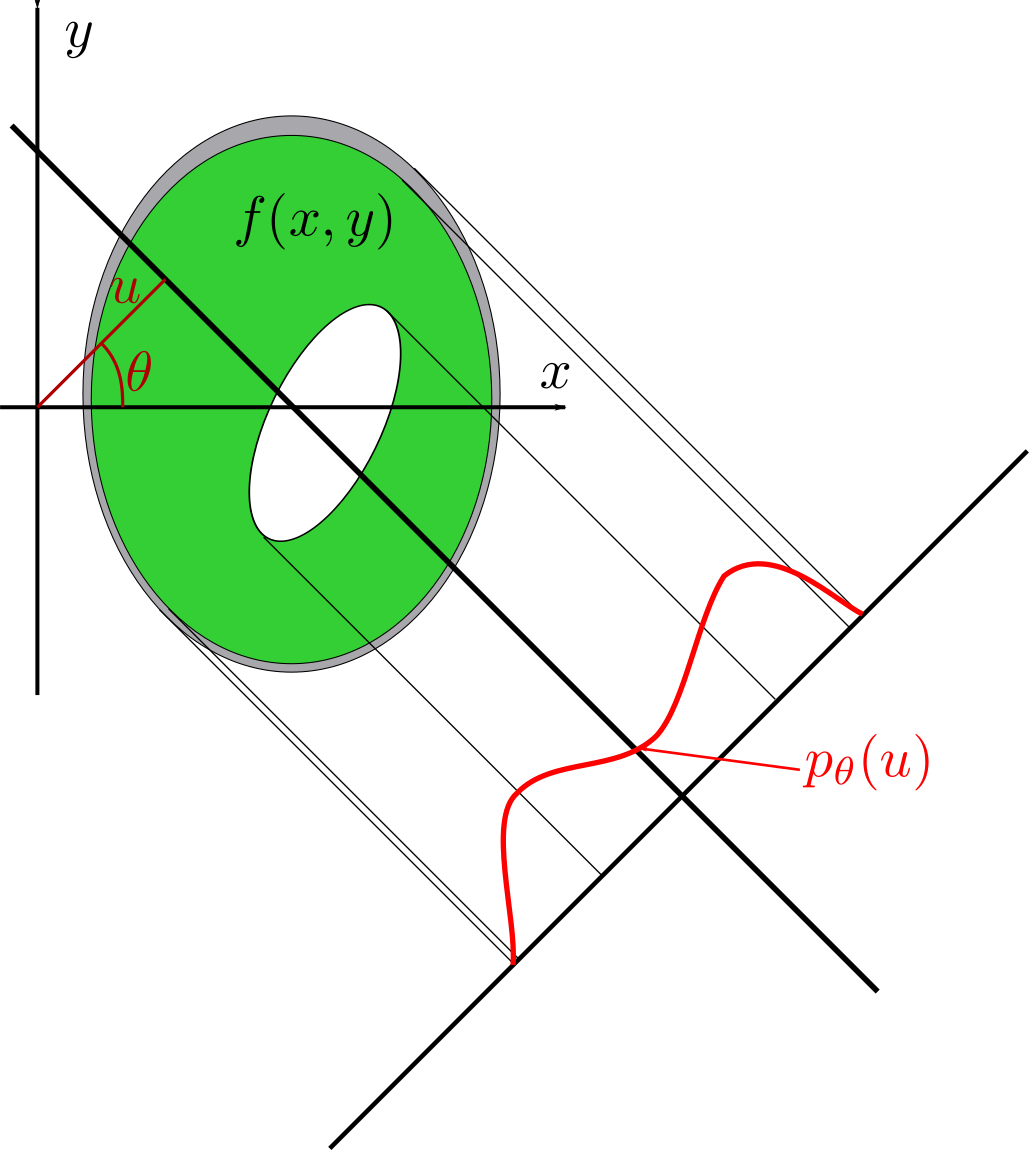
\includegraphics[width=8cm]{phantom.pdf}%
\end{figure}
An X-ray beam (considered as monochromatic) going through objects is attenuated, following a logarithmic law ($f$ is the linear attenuation, $v$ an elementary volume, $I$ the intensity of the beam entering the volume $dv$ and $I+dI$ the intensity exiting the volume):
$$\log \frac{I+dI}{I} = -fdv$$

By integrating this formula on a line $D$ (direction of the beam), yields:
$$I=I_0 \exp \left( \int_D f(x,y)dv \right) $$
where $f(x,y)$ is the attenuation at point $(x,y)$. This principle is used in scanners, scintigraphy, PET...

%\newpage
\section{Acquisition simulation}
This first exercise will allow us to simulate the projections. The mathematical operator behing this is the Radon transform.
\begin{qbox}
\begin{itemize}
 \item Generate a ``phantom'' image of size $256\times 256$. Display it. Notice that any image may be good for testing the simulation and reconstruction via backprojection.
 \item To simulate the attenation process, considere the sum of all gray levels of all pixels. Angles of projections will be between $0$ and $180$ degres with a unit step. The result is presented as a sinogram $p_\theta(u)$ (see Fig. \ref{fig:tomography:enonce:sino}), with $u$ the length (in ordinates), and $\theta$ the projection angle (in abscissa).
\end{itemize}
\end{qbox}

\begin{mcomment}
\begin{mremark}
Use the \matlabregistered{} function \minline{phantom}.
\end{mremark}
\end{mcomment}


\begin{figure}[htbp]
 \centering\caption{Simulated sinogram of the phantom image.}%
\subfloat[Sinogram.]{\includegraphics[height=5cm]{sinogramme.png}}
\hspace*{1cm}
\subfloat[Phantom image.]{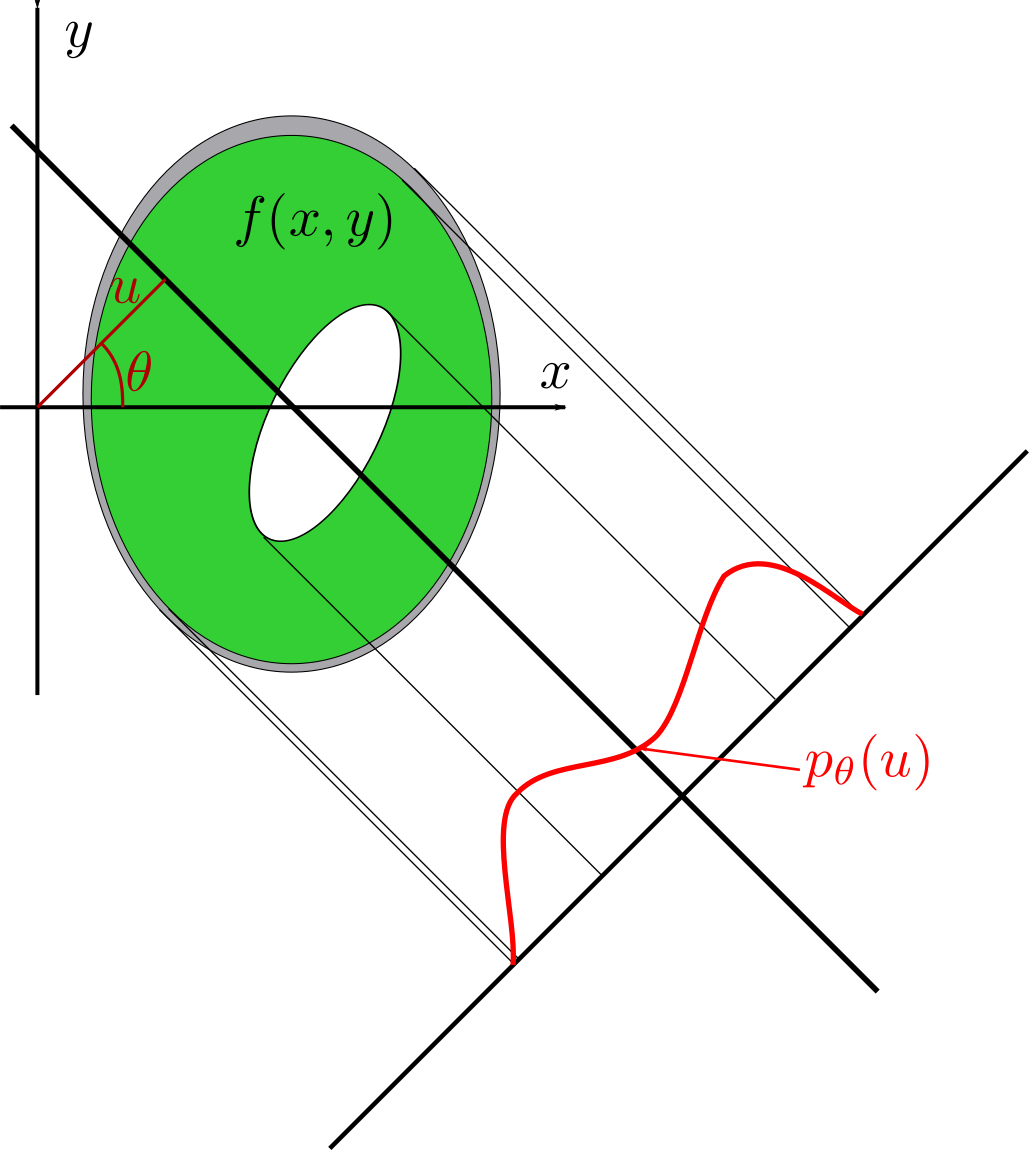
\includegraphics[height=5cm]{phantom.png}}%
\label{fig:tomography:enonce:sino}%
\end{figure}



\section{Backprojection algorithm}\index{Tomography!Backprojection}
A non exact reconstruction is the backprojection operator $B$ (it is not the inverse Radon transform). It attributes the value $p_\theta(u)$ to each point of the projection line that gave this attenation, and sum up all contributions from all projections (at the different angles).

$$B[p](x,y)=\int_0^\pi p_\theta(x\cos\theta+y\sin\theta)d\theta $$

A simple (but slow) method is described to compute the backprojection.
$p_\theta$ is the attenuation vector for a given angle $\theta$.
\begin{itemize}
 \item  Use a command to replicate a matrix to obtain the contribution of each line $D$, like on Fig. \ref{fig:tomography:enonce:contri}.
\begin{figure}[htbp]
\centering\caption{Backprojection}%
 \subfloat[Contribution of a line $D$ before rotation.]{\includegraphics[width=.45\linewidth]{contri.png}\label{fig:tomography:enonce:contri}}
\hfill
\subfloat[Reconstruction after pro\-jec\-tion every 45 degrees (4 pro\-jec\-tions).]{\includegraphics[width=.45\linewidth]{rec45.png}\label{fig:tomography:enonce:rec45}}%
\label{fig:tomography:enonce:retroprojection}%
\end{figure}
 \item Each contribution line $D$ should be turned of a certain angle to be added to the overall contribution. This backprojection is really fuzzy compared to the original phantom image (see Fig. \ref{fig:tomography:enonce:rec45}).
\end{itemize}

\begin{mcomment}
\begin{mremark}The function \minline{repmat} replicates a matrix a certain number of times.
\end{mremark}
\end{mcomment}

\section{Filtered backprojection}\index{Tomography!Filtered Backprojection}
It can be shown that backprojection is in fact the convolution of $f$ by a filter. A solution would be to make a deconvolution in the Fourier domain. The solution used here is the filtered backprojection. 

Numerous filters can be used. Among them, the Ram-Lak filter $RL$ is approximated by~:
\begin{eqnarray*}
 k\in[-B;B]\subset \N,  RL(k)           &=& \frac{\pi}{4}      \textrm{ if } k=0 \\
                              &=& 0                  \textrm{ if } |k| \textrm{ is even} \\
                              &=& \frac{-1}{\pi k^2}  \textrm{ if } |k| \textrm{ is odd}
\end{eqnarray*}

\begin{qbox}
\begin{itemize}
\item 
Write a function that generates this filter (see prototype). The parameter $width$  is the number of points  of the resulting vector.

\item Modify the backprojection algorithm to filter (by convolution of the projection vector) each contribution line before the summation. Observe the improved result.

\end{itemize}
\end{qbox}

\begin{mcomment}
\begin{mremark}

\begin{itemize}
\item Define a function with prototype: \minline{function ramlak = RamLak(width)}.
 \item MATLAB has builtin functions \minline{radon} and \minline{iradon} for projection and filtered backprojection algorithms. Test them.
\end{itemize}

 
\end{mremark}
\end{mcomment}


